\cotefile{157-3}
\scanpage{327}
% slanted
\margin{Cf pages 11~\unsure{ff|ss} pour \unsure{les} contreexemples-clef}

\uline{\unsure{Prop\textsuperscript{n}|Prop}} (?). Soit $X$ dans $\mathrm{Cat}$, \unsure{’un|un|ou} $b,c$ dans $X$ tels que

a) $b\times c$ est dans $X$

b) $\forall x$ dans $X$, $b(x)\ (\overset{\text{déf}}{=}\operatorname{Hom}_{X}(x,b))$ et $c(x)$ sont $\ne\emptyset$, i.e. $X_{/b}\longrightarrow X$ et $X_{/c}\longrightarrow X$ sont surj. sur les objets.

Alors $X$ est $W_\infty$-asphérique.

\margin{Faux, cf plus bas. $X$ est 1-connexe, mais pas néc. 2-connexe.}

Le fait que $b$ soit un plus grand élément de $\mathrm{Ob}\,\unsure{\alpha|X}$ assure déjà la 0-connexité.

Pour la 1-connexité, prouvons que dans le groupoïde fondamental $\Pi(X)$, $a\overset{\text{déf}}{=}b\times c$ devient un élément final. Pour ceci, prouvons \unsure{d'abord|s'abord} que $\forall x$ dans $X$, \deleted{\unsure{dans}} les éléments de $a(x)=b(x)\times c(x)$ sont égaux dans $\mathrm{Fl}\,\Pi(X)$. En effet, comme $b\times c\longrightarrow b$ est iso \inserted{ou \unsure{inverso|verso}} dans $\Pi(X)$, \unsure{cel|cela}

\diagram{\begin{tikzcd}[ampersand replacement=\&]
 b\times c \arrow[r]\arrow[d] \& b\\
 c \&
\end{tikzcd}}

montre déjà que \deleted{\unsure{soit}} si $\beta,\beta'\in b(x)$, $\gamma,\gamma'\in c(x)$, \deleted{$(\unsure{\beta},\unsure{\beta}),(\unsure{\beta'},\unsure{\gamma'})$} \inserted{\unsure{d'où} $(\beta',\gamma')$} $\in b(x)\times c(x)$, on a $(\beta,\gamma)=(\beta,\gamma')$ dans $\Pi(X)$ \deleted{\unsure{aussi}} (puisque $\mathrm{pr}_1(\beta,\gamma)=\mathrm{pr}_1(\beta,\gamma')$, et de $\unsure{=|\text{même}}$ (en utilisant que $\mathrm{pr}_2$ est iso dans \unsure{même}) $(\beta,\gamma')=(\beta',\gamma')$.

Donc tous les $(\beta,\gamma)$ \deleted{\unsure{deviennent}} \inserted{$\in b(x)\times c(x)=a(x)$} sont égaux dans $\mathrm{Fl}\,\Pi(X)$. Pour achever de prouver que $a$ est objet final de $\Pi(X)$, il suffit de voir que toute flèche \uline{dans} $\Pi(X)$ d'un $x\in\mathrm{ob}\,X$ dans $a$, provient d'une flèche $x\longrightarrow a$ dans $X$.

Mais une \deleted{telle} flèche \inserted{de $\Pi(X)$} est donnée par un chemin \deleted{dans} $X$

\diagram{\begin{tikzcd}[ampersand replacement=\&,column sep=small]
 x=x_0\arrow[r,"u_1"]\arrow[dr,"\alpha_0"'] \& x_1\arrow[d,"\alpha_1"] \& x_2\arrow[l,"u_2"']\arrow[r]\arrow[dl,"\alpha_2"] \& \dots \& x_{2N}=a\arrow[l,"u_{2N}"]\\
 \& a \& \& \&
\end{tikzcd}}

\deleted{\unsure{en}} prenons une flèche $\alpha_0:x\longrightarrow a_0$ dans $X$, je dis que \unsure{la|les}

% archive sheet number: 327
\scanpage{328}
\mspage{29}

je n'ai eu connaissance de l'Enterrement qu'en avril 1984, au bout de 14 ans...) Et rares ont été ceux parmi mes anciens amis qui, ayant senti ces effluves, ne s'en soient réjouis en leur for intérieur et n'aient fait chorus à la dérision dont j'étais l'objet. Ce faisant, ils croyaient qu'à toutes fins pratiques, le plaisir qu'ils y prenaient n'existait pas, puisque personne ne le voyait ni ne pouvait le prouver. En quoi ils se trompaient : car Dieu le voyait mieux qu'ils ne le voyaient eux-mêmes. Et Dieu n'a besoin d'aucune preuve pour conclure et pour agir.

7. Sens de l'Enterrement (3) - ou les coups bas

Je crois entrevoir une deuxième raison pourquoi Dieu a voulu que ma propre infidélité durant vingt ans soit suivie d'une infidélité (d'une durée égale - le hasard fait bien les choses...) du plus doué et du plus prestigieux parmi mes élèves. Comme je l'explique longuement dans Récoltes et Semailles, la relation entre cet élève et moi fut une sorte d'affinité élective, une ``lune de miel'' intellectuelle, une communion parfaite dans une passion de connaissance commune, d'une qualité si rare et (surtout) si haute, que l'idée qu'elle pourrait se dégrader jamais m'aurait en ces temps-là paru insensée et quasiment sacrilège ! Or, avec le recul et par un examen patient et obstiné, j'ai pu me rendre compte que dès ces temps idylliques d'une amitié qui semblait sans tâche ni fêlure, le ver déjà était dans le fruit, tant en moi, l'aîné, qu'en lui. En lui comme en moi, ce ``ver'' provenait des pulsions de l'égo qui, à l'abri du regard, sont à l'affut sans cesse pour faire feu de tout bois. Tant que les regards de l'un et de l'autre restaient absorbés par la fascination des ``choses de l'esprit'', ces pulsions cachées pouvaient en prendre à leur aise, pour se déclencher en actes à la première bonne occasion venue.

Mais, dans une relation à autrui, faire attention aux pulsions secrètes de la psyché que celle-ci met en jeu, tant en soi-même (en tout premier lieu) qu'en l'autre, est une \textit{vigilance} de l'âme, d'une essence plus subtile que les dispositions suscitées par la seule pulsion de connaissance intellectuelle (ou artistique, ou amóureuse, le cas échéant...).

Ainsi à mes yeux la mésaventure de mon élève et ami avec moi, et la mienne avec lui, illustre dans un cas particulièrement extrême, dans un cas qui peut passer pour ``idéal'', une vérité essentielle et universellement négligée, \textit{concernant toutes les relations humaines : c'est\unsure{,} qu'en l'absence d'une telle vigilance, d'essence spirituelle, qui naît d'une maturité et qui la promeut à son tour, les relations en apparence même les plus sûres ou les plus anodines, qu'elles soient basées sur des liens intellectuels} (comme ce fut le cas avec mon jeune ami), \textit{ou affectif, ou amoureux, ou de toute autre nature quels qu'ils soient, sont une source infinie de conflits sans issue.} Il en est ainsi, en tous cas, dès qu'une relation est assez forte pour (hem, hem...) pouvoir alimenter une envie de faire des vacheries ou de faire servir l'autre à ses fins, et pendant un temps suffisant pour que (hem, hem...) de telles envies aient le loisir au moins de se concrétiser en actes juteux et substantiels !

Ainsi cette ``mésaventure'' rocambolesque, débarassée de son grinçant par un ``happy end'' édifiant que Dieu tient en réserve pour très bientôt, m'apparaît comme une semonce magistrale de Dieu pour inculquer aux hommes cette ``vérité essentielle'' que je viens de dire et par là-même le sens très concret de la recommandation socratique (souvent citée, et très rarement comprise) du ``\textit{connais-toi toi-même}''.

% archive sheet number: 328
\scanpage{329}
\mspage{2}

classe d'homotopie \unsure{du chemin|des chemins} $c$ (i.e. son image dans $\mathrm{Fl}(\Pi(X))$ est égale à celle de $\unsure{u_0|\alpha_0}$. Pour le voir, choisissons pour \unsure{tt|tout} $i\in[0,\unsure{2N|N}]$ une flèche $\alpha_i:x_i\longrightarrow a$ \unsure{.} (ça existe grâce à l'hypothèse b)).

Je dis que pour chaque $i\in[0,2N]$, le triangle

\diagram{\begin{tikzcd}[ampersand replacement=\&]
 x_0\arrow[rr,"c_i"]\arrow[dr,dash,"\alpha_0"'] \& \& x_i\arrow[dl,dash,"\alpha_i"]\\
 \& a \&
\end{tikzcd}}

dans $\Pi(X)$ est commutatif, où $c_i$ désigne la classe d'homotopie du chemin de $x_0$ à $\unsure{x_i|x}$ défini par les $u_i$ ($i\in[1,i]$). Nous le faisons par récurrence sur $i$, \deleted{de sorte qu'on est} \inserted{l'assertion est} triviale si $i=0$ ($c_0$ représente l'application identique.)

\unsure{Le|On} \deleted{\unsure{est|a|un}} diagramme

\diagram{\begin{tikzcd}[ampersand replacement=\&,column sep=small]
 x_0\arrow[r,dash,"c_i"]\arrow[rr,dash,bend left=18,"c_{i+1}"]\arrow[dr,"\alpha_0"'] \& x_i\arrow[r,"u_{i+1}"]\arrow[d,"\alpha_i"] \& x_{i+1}\arrow[dl,"\alpha_{i+1}"]\\
 \& a \&
\end{tikzcd}}

montre qu'il suffit de prouver que pour $i\in[0,2N-1]$ le triangle

\diagram{\begin{tikzcd}[ampersand replacement=\&]
 x_i\arrow[rr,dash,"u_{i+1}"]\arrow[dr,"\alpha_i"'] \& \& x_{i+1}\arrow[dl,"\alpha_{i+1}"]\\
 \& a \&
\end{tikzcd}}

est commutatif dans $\Pi(X)$. (\uline{NB} $u_{i+1}$ est en sens direct ou rétrograde, suivant que $i$ est pair ou impair.) Mais cela résulte du fait que \deleted{\unsure{Hom}} l'image de $\operatorname{Hom}_X(x_{\unsure{i|1}},a)$ (resp $\operatorname{Hom}_{\deleted{\unsure{X}}X}(\unsure{x_{i+1}},\unsure{?|a})$

% archive sheet number: 329
\scanpage{330}
\mspage{30}

8. L'infidélité est un état d'abdication de l'âme

L'état d'infidélité doit être vue comme un état de maladie de la psyché, un état où l'être n'est pas véritablement lui-même. La vérité de l'être, celui qu'aux yeux de Dieu nous sommes vraiment, réside (et, sous des conditions favorables se développe) dans les couches profondes de la psyché, celles où le regard et les pulsions de l'égo n'ont plus accès. Ces couches font partie de l'âme proprement dite. La très grande majorité des personnes (et parmi elles quasiment tous les destinataires de la Lettre) ignorent totalement l'existence de leur âme, de ce qui est véritablement et profondément ``eux'', à l'exclusion du bruit confus et du bric-à-brac à tout venant qui encombre (au point souvent de les étouffer) les couches moyennes et superficielles. Ceux qu'on appelle communément ``les croyants'' n'y font généralement pas plus exception que les autres. Comme ``tout le monde'', ils s'identifient plus ou moins totalement à leur égo, la seule partie de leur psyché (à part tout au plus la pulsion amoureuse) dont ils se soient jamais souciés de prendre connaissance. Ce que communément on bâptise du nom bien sonnant d'``esprit'' ou d'``âme'', n'est le plus souvent qu'une pose de l'égo, arborée aux grandes occasions, quand on pavoise à la ``spiritualité''. C'est là, le plus souvent, l'effet d'une simple ignorance spirituelle, donc d'une certaine immaturité. Mais fort heureusement l'immaturité n'empêche nullement l'âme d'être fidèle. \textit{L'âme même la plus frustre a toujours les moyens d'être fidèle, c'est-à-dire aussi, d'être vraie.}

L'état de fidélité, qui n'est autre chose qu'un état d'authenticité minimum de l'être, est celui où la connaissance et les pulsions d'action des couches profondes parviennent à la surface, vers la conscience, au moins partiellement et avec une certaine efficacité, pour s'y exprimer en connaissance, en pensées, en perceptions et sentiments, et en actes. L'état d'infidélité est celui où la communication entre les couches profondes et la surface de la psyché est plus ou moins totalement coupée, quand les couches créatrices profondes ont cessé de stimuler et de nourrir l'activité totale de la psyché. C'est comme un état d'asphyxie de l'âme : l'âme étouffe...

Ce blocage dans la communication entre couches profondes et couches superficielles \textit{est toujours l'effet d'une action de l'égo.} Il n'est d'ailleurs nullement dans la nature éternelle de l'égo d'agir ainsi, comme une force d'asphyxie. L'égo doit assurer dans la psyché des fonctions d'intendance indispensables, qui ne cessent nullement après la libération de l'âme. Sa propension à agir comme une force de blocage, tout comme sa propension à une hypertrophie sans limites, peuvent être vues comme des aspects cruciaux de la ``\textit{maladie d'enfance}'' de l'âme, au cours de son errance de naissance en naissance, maladie qui ne prend fin qu'avec l'Acte de libération. Pour être précis, c'est là plutôt une \textit{maladie de l'égo}, non de l'âme elle-même ou de la psyché dans sa totalité. En fait, une des principales responsabilités de l'âme est la \textit{vigilance vis-à-vis de l'égo}, pour veiller à ce que celui-ci ne se substitue à elle pour diriger la psyché et pour exercer un contrôle plus ou moins total sur les actes. L'état de blocage dont il vient d'être question n'est autre que celui où l'âme a renoncé plus ou moins totalement à son rôle d'instance dirigeante et responsable dans la psyché, pour abdiquer de ces prérogatives au bénéfice de l'égo. Etat d'inauthenticité, état d'asphyxie, état de blocage, l'infidélité peut donc être vue aussi comme un \textit{état d'abdication} : avec et par le consentement de l'âme, l'état de maladie congénitale de l'égo (sa ``maladie d'enfance'') a désormais gagné l'ensemble de la psyché.

% archive sheet number: 330
\scanpage{331}
\mspage{3}

dans \deleted{$\operatorname{Hom}_{\Pi(X)}$} $\mathrm{Fl}\,\Pi(X)$ est réduite à un seul élément.

Ainsi on trouve que \uline{$X$ est 1-connexe}. Il y a donc de l'espoir ! Il reste à prouver

\[
 H^i(X,M)=0 \qquad i\geq 2,\quad M\ \text{coeff. const.}
\]

J'\deleted{\unsure{y}}ai \deleted{vérifié lorsque $b=c$, et \unsure{on}} \inserted{regardé le cas lorsqu'on} a ceci : $b=c$, $\mathrm{Ob}\,X=\{b,b\times b\}$, $\operatorname{Hom}_X(b\times b)=\{\text{réunion disjointe des ens }u\circ\mathrm{pr}_1\text{ et }u\circ\mathrm{pr}_2,\text{ où }u\in\operatorname{Hom}_X(b,b)=G,\text{ un monoïde quelconque.}$ \deleted{\illegible{1}} \deleted{Alors} \inserted{\unsure{Ici}} $X^{\unsure{\circ|o}}$ est \deleted{\illegible{1}} fibrée, \inserted{via $I\mapsto b^I$,} sur la \inserted{sous} catégorie pleine \inserted{$S$} de Ens formée de $\{0\}$ et $\{0,1\}$, et

\[
 \deleted{H^n(X,M)\simeq H^0(S,\mathscr H^n)\quad\unsure{\text{or ici}}}
\]

\deleted{et on vérifie \inserted{surtout} que c'est nul pour $n\geq 1$. (NB. les $H^p(S,\unsure{\mathscr H^q})$ sont nuls pour $p>0$, car $S$ a $\{0\}$ comme objet final. \unsure{Si}...} Donc $X$ est cofibrée (\deleted{\unsure{sur}} \unsure{potentiellement|particules|parties} propres) sur $S^\circ\overset{\text{déf}}{=}T$. (NB. $\unsure{S^\circ|S^0}=T$ a un objet initial, mais non un objet final. Sa \unsure{coh.|cat.} à val. dans un préfaisceau quelc. \unsure{n'est} pas \unsure{tjs} \deleted{\unsure{bien connu}} triviale, cf ci dessous)

\[
 H^n(X,M)\Longleftarrow H^p\bigl(T,\underbrace{R^q f_*(M_X)}_{=\mathscr H^q}\bigr)
 \qquad \text{où }f:X\unsure{\text{---}|\longrightarrow} S^\circ .
\]

J'admet ici (provisoirement) ceci :

\[
 \begin{aligned}
 \deleted{\unsure{\forall}}\ H^p(\deleted{\unsure{S^\circ}}T,\deleted{\unsure{\mathscr H^q|R^q}}F)&=0\qquad\text{pour }p\geq2,\ \text{tout }F\in T^\wedge.\\
 H^0(T,F)&\simeq\operatorname{Ker}\delta\\
 H^1(T,F)&\simeq\operatorname{Coker}\delta
 \end{aligned}
\]

\margin{où $\delta:F_0\longrightarrow F_1$ est défini comme la différence $\delta=p_1^*-p_2^{\unsure{*|-}}$}

\margin{où $p_1,p_2$ sont les deux proj. de $\{0,1\}\simeq\{0\}^2$ dans $T^{\unsure{\circ}}\!=S^\circ$}

\deleted{On vérifie de plus} \inserted{On a de plus}

\[
 (\mathscr H^q)_0=H^q(G,M),\quad (\mathscr H^q)_1=H^q(G\times G,M)
\]

et

\[
 \mathrm{pr}_1^*,\mathrm{pr}_2^*:H^q(G,M)\rightrightarrows H^q(\unsure{G\times G},M)
\]

sont les \unsure{transposés|transportés|transposées} de $\mathrm{pr}_1,\mathrm{pr}_2:G\times G\longrightarrow G$

% archive sheet number: 331
\scanpage{332}
\mspage{31}

A l'opposé des infirmités congénitales de l'égo, un tel état de maladie de la psyché et de l'âme n'est nullement une désolante fatalité. Ce n'est pas notre état lors de notre naissance sur terre, et il ne s'instaure jamais sans qu'il n'y ait de la part de l'âme un acte ou des actes à cet effet (dont la portée le plus souvent reste inconsciente). Ce sont les ``\textit{actes d'infidélité}'', lesquels (en tenant compte de la subreptice immixtion de l'égo partout dans la psyché...) ne sont ni plus, ni moins que les \textit{actes d'abdication} plus ou moins complète de l'âme devant la poussée envahissante de l'égo. Et aux yeux de Dieu, l'acte le plus grave de tous que l'âme puisse commettre, c'est l'acte d'abdication totale. (Et un tel acte est toujours une abdication \textit{au profit de l'égo}.) C'est cela et rien d'autre qu'il faut entendre par ``\textit{suicide spirituel}''.

Parmi les destinataires de la Lettre, il en est plus de vingt qui sont à l'état de cadavres spirituels. Mais en eux, comme en tous les autres, Dieu agira. Il les arrachera malgré eux à leur mort volontaire. Et les morts vivront, et marcheront...

9. L'infidélité est un état de vanité

Ce qui constamment pèse sur l'âme avec plus ou moins d'insistance ou de véhémence et qui constamment la pousse aux actes d'infidélité, ce sont les poussées issues de la \textit{vanité}, ou de la forme ``dure'' de celle-ci : \textit{l'orgueil}, et le \textit{désir de domination} qui très souvent en découle. \textit{La ``maladie d'enfance'' dont il vient d'être question, maladie de l'égo qui sans cesse tend à envahir toute la psyché, n'est autre que la vanité.} Et cette maladie gagne l'âme, l'âme est ``infidèle'', dès l'instant où elle s'abandonne yeux fermés aux pulsions de vanité provenant de l'égo. Et \textit{tous} ses conditionnements sans exception, tant familiaux que culturels et y compris même (sous une forme parfois plus subtile) les conditionnements ``religieux'', poussent l'âme depuis sa plus tendre enfancé dans la voie d'une telle abdication.

Aussi la vanité est-elle, et de très loin, la maladie la plus répandue parmi les hommes. Et la psyché a été réglée par Dieu de telle façon qu'elle ne voit la vanité pratiquement jamais que chez autrui (chose facile, et qui rarement nous avance à grand chose...). Aussi celui qui a franchi le pas de reconnaître enfin cette maladie tenace en lui-même, et qui dans la joie de son coeur se hasarde à parler de sa grande découverte, se voit aussitôt traité avec des airs de commisération condescendante, coupant court aussitôt à toute velléité de communication...

A la bonne heure, certaines lectures m'avaient mis en tête l'idée (consolatrice et des plus convaincantes...) que dès lors qu'on a clairement reconnu la présence envahissante de la vanité dans sa psyché, tout était fait et que ladite vanité allait, sous ce regard scrutateur, s'évanouir comme par enchantement. Cela fait plus de treize ans à présent que je scrute, sans en être débarassé pour autant. Il est vrai qu'aussi longtemps qu'on tient la garce à l'oeil, elle se tient plus ou moins à carreau. (Mais gare aux moments d'inattention !) Ce qui est sûr, c'est qu'en moi elle a cessé de faire la loi. Et c'est beaucoup...

Mais pour tous ceux à qui s'adresse la Lettre, un tout premier pas à franchir pour reconnaître son état d'infidélité et pour y mettre fin, c'est de prendre connaissance de l'action de la vanité dans son être. Des \textit{résistances} occultes d'une force immense, sur le qui vive à toute heure tant dans l'égo que dans l'âme, s'opposent efficacement à une telle prise de

% archive sheet number: 332
\scanpage{333}
\mspage{4}

On vérifie aisément que

\[
 H^0(T,\mathscr H^q)=0\qquad\text{si }q\geq1
\]

et il reste

\[
 \begin{aligned}
 H^n(\deleted{\unsure{T}}X,M)&\simeq H^1(S,\mathscr H^{n-1})=\operatorname{Coker}\bigl(\delta:H^{n-1}(G)\longrightarrow{}\\
 &\hspace{12em}H^{n-1}(G\times G)\bigr)
 \end{aligned}
\]

Cela donne, pour $n=2$

\[
 \begin{aligned}
 H^2(X,M)&\simeq\operatorname{Coker}\bigl(\delta:\operatorname{Hom}_{\mathrm{mon}}(G,M)\longrightarrow
 \underbrace{\operatorname{Hom}_{\mathrm{mon}}(G\times G,M)}_{\operatorname{Hom}_{\mathrm{mon}}(G,M)\times\operatorname{Hom}_{\mathrm{mon}}(\unsure{G,M})}\bigr)\\
 &\simeq\operatorname{Coker}\bigl(u\longmapsto(u,-u):H\longrightarrow H\times H\bigr)
 \end{aligned}
\]

où $H$ est le groupe abélien $\operatorname{Hom}_{\mathrm{mon}}(G,M)$.

D'où

\[
 H^2(X,M)\simeq H=\operatorname{Hom}_{\mathrm{mon}}(G,M).
\]

Donc $X$ est 2-connexe \unsure{sss|ssi} lé groupe \uline{abélien} enveloppant du monoïde $G$ est nul.

Ainsi, si $G$ est un groupe abélien $\ne0$, $X$ n'\uline{est pas} 2-connexe.

\deleted{Conjecture} \uline{\unsure{Corollaire|Conclusion}} $\deleted{\unsure{\mathscr D}}\unsure{\Psi|\mathscr V|V}={}$

\diagram{\begin{tikzcd}[ampersand replacement=\&,row sep=tiny]
 \& b_0\\
 a_0\arrow[ur]\arrow[dr] \&\\
 \& c_0
\end{tikzcd}}

n'est \uline{pas} \deleted{\unsure{tot.}} $W_\infty$-asphériseur ; i.e. si on a un diagramme

\diagram{\begin{tikzcd}[ampersand replacement=\&,row sep=tiny]
 \& b\\
 a\arrow[ur]\arrow[dr] \&\\
 \& c
\end{tikzcd}}

dans une cat. $X\in\mathrm{Ob}\,\mathrm{Cat}$, telle que \unsure{sa|de} somme amalgamée dans $X^\wedge$ soit égale à $e_X$, il ne s'ensuit pas que $X$ soit $W_\infty$-asphérique, (Mais \deleted{\unsure{semble}} peut-être $X$ \unsure{voudra|doive} bien être 1-connexe ?)

% archive sheet number: 333
\scanpage{334}
\mspage{36}

Quand l'une après l'autre les quatre dépendances fondamentales, par rapport à la Mère, par rapport à l'Epouse, par rapport au Père, par rapport à l'Epoux ont été dissoutes, toutes les racines de la vanité dans la psyché sont désormais coupées. \textit{La vanité est morte.} Les mécanismes et les comportements vaniteux dépérissent rapidement et disparaissent, sans plus laisser de traces. La tentation vaniteuse disparue, plus jamais l'âme ne sera infidèle. Elle est prête désormais pour l'Acte de libération - pour la libération totale qui met fin à son état d'errance, la faisant entrer à jamais dans l'état de liberté.

Ces éclaircissements placent dans une perspective nouvelle et saisissante la promesse de Dieu, de veiller à ce que dans les jours déjà qui suivent Son appel, dès cette année donc, vous résolviez totalement votre ``problème aux parents''. Par là il faut entendre, plus précisément, qu'au terme d'un travail assidu que vous accomplirez alors, Il mettra fin à votre dépendance aussi bien par rapport à la Mère, que par rapport au Père. Ce sera la fin de la ``\textit{guerre des générations}'' dans votre psyché. Il faut noter ici, de plus, que dans le mécanisme psychique originelle, la dépendance par rapport aux Figures parentales joue presque toujours un rôle prépondérant vis-à-vis de celle par rapport aux Conjoints. C'est dire que la promesse de Dieu peut aussi se reformuler ainsi : \textit{Dieu se propose de vous libérer, dès cette année-ci, du plus gros de votre dépendance invétérée} (pesant sur vous depuis l'origine des Temps) \textit{par rapport aux mécanismes de la vanité.}

Pour peu que par la suite vous persévériez dans un effort de connaissance de soi, Dieu est même décidé à faire fructifier très rapidement votre effort, en vous libérant de vos deux autres dépendances archétypes, celles par rapport à l'Epouse et à l'Epoux. Cette fois, ce sera la fin de la ``\textit{guerre des sexes}'' dans votre âme. Du même coup, ce sera aussi la fin de ce qui restait en vous de vanité.

Ainsi, grâce à l'état d'exception du ``\textit{Temps de la Fin}'' précédant l'avènement du Nouvel Age, et grâce à la mission de messager que Dieu entend vous confier, vous vous trouvez placé devant l'inimaginable option de parvenir, par un travail limité à des semaines ou à des mois sans plus, à un état de maturité spirituelle et de liberté intérieure hors du commun. Un état auquel l'âme ne parvient généralement (à partir du point où vous en êtes à présent, et quand elle y parvient bel et bien pendant l'Age de l'Errance) qu'au terme de centaines ou de milliers d'existences.

Moi-même puis témoigner à cet égard que tout au cours des treize années écoulées, j'ai investi un maximum d'efforts de vigilance et de réflexion sur moi-même, dans l'espoir de me libérer de la vanité. Mon seul succès a été de la voir toujours plus clairement - et toujours aussi florissante !

Quant à vous qui aurez dans vos voiles un Vent plus efficace que celui dont jusqu'à présent j'ai pu bénéficier, une fois entré dans votre mission et animé par l'esprit du Nouvel Age, vous ne pourrez vous empêcher de persévérer dans un effort de connaissance de soi et d'approfondissement. A ce compte, d'ici quelques années déjà, poussé par le Souffle de Dieu, vous aurez mûri au point d'être prêt pour l'Acte de libération. Et avec joie et sans attendre un jour de plus Dieu accomplirait l'Acte, s'Il n'était retenu par les lois spirituelles qu'Il a lui-même instaurées, et qui mettent des limites à l'aide qu'Il peut accorder au cours d'une seule existence terrestre. Aussi, sauf pour un très petit nombre parmi ceux à qui je m'adresse ici, votre libération ne se fera pas encore dans votre présente existence,

% archive sheet number: 334
\scanpage{335}
\mspage{5}

\uline{Question} Y-a-t-il d'autres objets \deleted{\unsure{tot.}} $W_\infty$-\unsure{asphérique|asphériques} de $\mathrm{Cat}$, que les catégories ayant un objet final ? Je suspecte à présent que non - donc que l'on ne peut améliorer \deleted{\unsure{substanti}} \unsure{ellement|tellement} sur la notion déjà connue d'immersion ouverte de Dwyer.

\figure{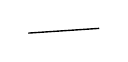
\begin{tikzpicture}\draw[line width=.5pt] (0,0) -- (.9,.06);\end{tikzpicture}}

Dans le diagramme

\diagram{$(\alpha)$\qquad\begin{tikzcd}[ampersand replacement=\&,column sep=large]
 U\arrow[r,hook,"i"]\arrow[d,dash,"p"'] \& X\arrow[d,dash,"q"] \& T\arrow[l,dashed,hook',"j"']\arrow[d,"\mathrm{iso}"]\\
 U'\arrow[r,hook,"i'"']\arrow[ur,phantom,"\text{\scriptsize cocart. et cart.}" description] \& X'\& T'\arrow[l,dashed,hook',"j'"]
\end{tikzcd}}

prenons $U=\Psi$, $T=\{t\}=e$ catégorie finale, $t$ objet final \deleted{de $X$} i.e. \deleted{$\unsure{E|H|\square}$}

\[
 H_t=\bigl(u\longmapsto\operatorname{Hom}_X(u,t)\bigr)=e_{\unsure{U|u}}\in\mathrm{Ob}\,U^\wedge
\]

% slanted
\margin{i.e. $X$ déduit de $U=\Psi$ en lui rajoutant un objet final $t$ donc $X\simeq\Delta^1\times\Delta^1$}

% slanted
\margin{\diagram{\begin{tikzcd}[ampersand replacement=\&,column sep=small,row sep=small,execute at end picture={\draw[rounded corners=5pt] ([xshift=-5pt,yshift=6pt]TL.north west) -- ([xshift=8pt,yshift=6pt]TL.north east) -- ([xshift=8pt,yshift=-8pt]TL.south east) -- ([xshift=6pt,yshift=8pt]BR.north east) -- ([xshift=7pt,yshift=-5pt]BR.south east) -- ([xshift=-7pt,yshift=-6pt]BL.south west) -- cycle;}]
 |[alias=TL]|\phantom{x}\arrow[r] \& \phantom{x}\\
 |[alias=BL]|\cdot\arrow[u]\arrow[r] \& |[alias=BR]|\phantom{x}\arrow[u]\\
 \Psi\arrow[u,shorten >=4pt] \&
\end{tikzcd}}}

Prenons pour $U'$ la cat. dont il est question dans la ``prop.'' hypothétique (et \unsure{fausse}) p 1, \inserted{avec $b=c$,} plus précisément une catégorie \deleted{\unsure{ab}} avec deux objets $b$ et $b\times b$, un groupe \inserted{(voire un monoïde)} $G$ d'endom. de $b$, et les autres flèches celles qui s'en \unsure{déduisent}, en exigeant que $b\times b$ soit bel et bien le carré cartésien de $b$. On trouve une catégorie cofibrée (\deleted{\unsure{non}} propre) sur la cat. $T$ opposée de celle des ens finis de la forme $\{0\}$ et $\{0,1\}$ (deux objets) avec comme fibres $B_G$ et $B_{G\times G}$ respectivement.

($B_{\unsure{\Pi|\pi|R}}:=$ cat. avec un seul objet, et monoïde d'endomorphismes $\unsure{R|\Pi|\pi}$.) Le foncteur \unsure{2|?}

\[
 U=\Psi\longrightarrow U'
\]

est celui donné par le diagramme

% archive sheet number: 335
\scanpage{336}
\mspage{37}

mais seulement au terme de la suivante. Pendant celle-ci, totalement libéré déjà des entraves de la vanité et de l'agressivité, vous aurez le rare privilège de servir alors pour la progression de tous les hommes plutôt que pour la vôtre, avec la coopération constante de Dieu et dans l'accomplissement d'une très grand mission qui vous aura été confiée par Lui.

14. La relation à nos parents domine notre vie

Dans ce que je viens de dire sur les racines de la vanité, il n'a été question que de l'aspect ``positif'' de la dépendance par rapport aux figures archétypes, à savoir du désir de leur plaire, ou celui de conquérir leurs faveurs. Ce désir conduit toujours à endosser des actes et des comportements qui ne naissent nullement des pulsions créatrices de l'être profond, mais de \textit{la soumission à des désirs supposés, toujours factices et toujours spirituellement stériles, que l'égo a été amené à prêter aux figures archétypes}, en réponse purement mécanique aux conditionnements reçus dans la présente existence et dans les existences précédentes. A dire vrai, il n'y a pas lieu de distinguer entre la Figure archétype elle-même, celle de la Mère disons, qui vit dans l'inconscient moyen, et cette \textit{image ``factice''} que l'égo se forme tout au cours du temps de l'errance, sous l'effet des divers conditionnements issus des circonstances de tout ordre qui entourent chacune de nos existences. Quant à l'archétype ``véritable'' de la Mère, on peut dire de lui qu'il est ``\textit{universel}'', c'est-à-dire qu'il est le même pour toutes les âmes. Il n'est la création ni de l'égo, ni de la psyché, ni même création de Dieu. Il existe en Dieu hors du temps, comme un des aspects éternels de Dieu : \textit{Dieu est Mère.} (Comme Il est aussi Père, comme Il est Epouse, comme Il est Epoux...) Et \textit{l'inconscient profond perçoit ``la Mère'' dans son essence véritable}, libre de toute déformation. C'est cette perception elle-même qui ``est'' la \textit{``véritable'' Figure archétype de la Mère, vivant, elle, dans l'inconscient profond et nourrissant ses pulsions créatrices tout au cours de nos existences} (tant terrestres, que dans l'au-delà). En elle réside la \textit{Réalité}, c'est-à-dire la perception véritable et fidèle que nous avons de la réalité. Cette Réalité est cachée plus que révélée par la \textit{Maya}, s'en donnant à coeur joie dans les couches moyennes et superficielles de la psyché, autour de l'image d'une ``Mère'' de pacotille (et parfois pas piquée de vers...).

Les conditionnements qui façonnent notre perception ``factice'' des Figures archétypes remontent presque tous à l'enfance. Ils sont déterminés en tout premier lieu par le milieu parental et par la relation des parents entre eux et à leur enfant (et, le cas échéant, à ses frères et soeurs). Sauf exceptions rarissimes, dues à des situations familiales exceptionnelles, \textit{les premiers êtres investis par les figures archétypes au cours d'une existence sont la mère, investie à la fois du rôle de} Mère \textit{et} d'Epouse, \textit{et le père, investi de même d'office du rôle de} Père \textit{et} d'Epoux. En l'absence de père ou de présence masculine en tenant lieu, la mère presque toujours se trouve investie également des rôles ardus (pour une mère...) et de Père, et d'Epoux. Et inversement dans le cas, de beaucoup plus rare, où le père doit suppléer à l'absence d'une mère défaillante.

Il faut se rappeler cependant que \textit{dès notre naissance}, en plus des \textit{Figures archétypes réelles} de la Mère, de l'Epouse, du Père, et de l'Epoux, qui vivent dans l'inconscient profond d'une existence éternelle et immuable, nous apportons déjà avec nous les \textit{figures archétypes factices} qui en sont un reflet déformé, et qui s'agitent dans l'inconscient moyen. Elles sont le produit surtout des conditionnements auxquels nous nous sommes trouvés soumis au cours de nos précédentes existences, et des réactions (le

% archive sheet number: 336
\scanpage{337}
\mspage{6}

\diagram{\begin{tikzcd}[ampersand replacement=\&,row sep=tiny]
 \& b\\
 b\times b\arrow[ur,"\mathrm{pr}_1"]\arrow[dr,"\mathrm{pr}_2"'] \&\\
 \& b
\end{tikzcd}}

dans $U'$, et les \unsure{hyp.|hypp.} \unsure{a)|b)}, b) de la page 1 assurent que la somme amalgamée \uline{dans} \unsure{de|des|du} ce diagramme \deleted{\unsure{du|de}}dans $U'^\wedge$ est $e_{U'}$, i.e. que

\[
 p_!(e_U)=e_{U'}.
\]

Il s'ensuit \deleted{\unsure{que}} ds la somme amalgamée $X'$ envisagée ds $(\alpha)$, l'unique élément $t'$ de $T'$ est objet final de $X'$. On a vu que $U'$ \deleted{\unsure{ne}} est 1-connexe, mais non 2-connexe si le groupe abélien enveloppant de $G$ (i.e. $G/$\inserted{groupe des} commutateurs dans le cas où $G$ est un groupe) n'est pas réduit à 1. L'exemple le plus économique s'obtient en prenant $G=\{\pm1\}$ le groupe à deux éléments. C'est donc un cas où dans \unsure{$(\alpha)$|cas} on a

\[
 \underset{\substack{\text{(et même}\\\text{asphérique)}}}{i\in W},\qquad \text{mais }i'\notin W,
\]

et qui a l'avantage sur l'exemple plus sophistiqué de la page \unsure{153|W3} (prop. \unsure{10|W}) de ne mettre en jeu que des catégories finies - et même fort petites !

Procédons maintenant comme dans la prop. 11, en désignant par $U''$ la catégorie déduite de $U'$ en lui ajoutant un objet

% archive sheet number: 337
\scanpage{338}
\mspage{38}

plus souvent purement mécaniques, mais par moments aussi créatrices) de la psyché à ceux-ci. Aussi les relations de l'enfant en bas âge à ses parents, dès avant même que les conditionnements propres à son présent milieu familial aient pu s'imprimer dans la psyché, sont dominées par ces figures archétypes ``factices'' de la Mère, de l'Epouse, du Père, et de l'Epoux qu'il a apportées avec lui ; tels des bagages lourds et encombrants, qu'il lui appartiendra d'alléger au cours de sa présente existence. Dès les premières années de l'enfance, ces archétypes factices se modifient dans un sens ou un autre sous l'influence du milieu parental et surtout, sous celle de la relation des deux parents à l'enfant. C'est dans ces années-là qu'ils prennent leur visage (le plus souvent) définitif, lequel reste plus ou moins immuable jusque dans la vieillesse. Durant tout l'Age de l'Errance, ce n'est que très exceptionnellement, dans une vie d'une fertilité spirituelle hors du commun, que l'un ou l'autre de ces visages s'affine et se décante, pour s'approcher de la Réalité.

En raison de l'importance cruciale des archétypes de la Mère et du Père, et de ceux de l'Epouse et de l'Epoux dans la vie de la psyché, \textit{notre relation à chacun de nos deux parents, et plus encore} (presque toujours) \textit{ce que fut cette relation pendant l'enfance, domine nos actes et nos comportements au cours de toute notre existence.} Il est bien entendu qu'il s'agit ici de la relation aux parents telle qu'elle est réellement, c'est-à-dire surtout de ce qui se passe dans l'inconscient moyen, et nullement de l'image toute plate et conventionnelle que nous nous plaisons à entretenir de cette relation.

De là découle d'une part, \textit{à quel point le rôle de parent est essentiel, à quel point la façon dont il est assumé ou négligé marque la vie entière de celui qui comme enfant fut confié entre nos mains.} Aussi parmi nos relations à autrui, c'est celle de parent à enfant qui, aux yeux de Dieu, implique la responsabilité la plus essentielle. C'est une responsabilité qui n'est pas éteinte par la mort de celui qui fut notre enfant. Elle accompagne celui-ci de naissance en naissance, jusqu'au moment de sa libération. (Par quoi s'éteint toute dette qu'une âme pouvait avoir à son égard...)

Mais d'autre part (et dans l'optique ``opposée'', de celui qui fut enfant), il découle de ceci à quel point il est essentiel pour l'âme, pour accéder à une maîtrise réelle de ses actes et à une véritable authenticité, d'arriver à résoudre son ``problème aux parents''. Cette tâche est inséparable de celle de clarifier notre relation tant à la mère qu'au père, en nous libérant des dépendances inconscientes par rapport à elle et à lui. De plus, en raison de la relation très forte qui relie l'un et l'autre parent non seulement aux archétypes parentaux, mais aussi à ceux du Conjoint, être libéré\deleted{e} (par Acte de Dieu) de sa dépendance par rapport aux Parents implique aussi, presque toujours, un affaiblissement de la dépendance aux archétypes de l'Epouse et de l'Epoux. Aussi une fois libérée de la ``guerre des générations'' dans sa psyché, l'âme est désormais en meilleure posture pour travailler à mettre fin aussi à la ``guerre des sexes'' qui se joue en elle.

15. La pulsion homosexuelle est une pulsion éternelle dans tout être humain

On ne peut trop insister sur cette loi fondamentale et universelle dans la vie de la psyché, que la \textit{mère est investie d'office non seulement de l'archétype de la Mère, mais aussi de celui de l'Epouse ; et de même le père est investi aussi, à côté de l'archétype ``anodin'' du Père, de celui de l'Epoux.} Cette loi, m'est-il assuré, est toujours obéie, elle ne souffre

% archive sheet number: 338
\scanpage{339}
\mspage{7}

final, et soit

\[
 p':\underset{\unsure{k|x|\downarrow}}{U'}\unsure{\mathbin{-}|\longrightarrow} U''
\]

l'inclusion, de sorte que

\[
 p'_!(e_{U'})=(p'p)_!(e_U)\unsure{=|\simeq} U'
 \quad\begin{gathered}\text{en tant qu'objet}\\
 \text{dans }U''^\wedge\ \text{(sans \deleted{\unsure{préf.}}\unsure{rapports|préf.}}\\
 \text{avec le préfaisceau}\\
 \text{final }e_{U''}\text{)}\end{gathered}
\]

Considérons

\diagram{\begin{tikzcd}[ampersand replacement=\&,column sep=large]
 U\arrow[r,hook,no head,"i"]\arrow[d,"p''=p'p"'] \& X\arrow[d,"q''"] \& T\arrow[l,hook',dashed,"j"']\arrow[d,"\mathrm{iso}"]\\
 U''\arrow[r,hook,"i''"']\arrow[ur,phantom,"\substack{\text{cocart.}\\\text{et cart.}}" description] \& X'' \& T''\arrow[l,hook',dashed,"j''"]
\end{tikzcd}}

Cette fois $U,X$ \uline{et} $U''$ sont $W_\infty$-asph. (et même contractiles toutes trois), \deleted{donc $i,p''$} \inserted{donc} $i,p''$ sont dans $W$, pourtant $X''$ n'est pas $W_\infty$-asph. (donc $i'',q''\notin W_\infty$), car pour qu'\unsure{el|il}\deleted{\unsure{le}} le soit \inserted{i.e. pour que $\unsure{i''|i'''}\in W_\infty$,} il faudrait (prop. 7, \unsure{cor|ou} page $85^*$) que \inserted{$i''$ soit \unsure{loc.|hom.} asph., i.e.} $U''_{/t''}$ soit $W_\infty$-asphérique. Mais par construction $U''_{/t''}\simeq U'$, qui n'est \uline{pas} $W_\infty$-asphérique.

% slanted
\margin{pas encore démontré !}

\figure{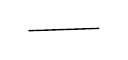
\begin{tikzpicture}\draw[line width=.5pt] (0,0) -- (.9,.03);\end{tikzpicture}}

Voilà un exemple encore plus simple d'un foncteur $f:\Psi\longrightarrow X$ tel que $f_!(e_\Psi)$ ne soit pas $W_\infty$-asphérique, \deleted{L'idée} i.e. d'un diagramme

\diagram{\begin{tikzcd}[ampersand replacement=\&,row sep=tiny]
 \& b\\
 a\arrow[ur,"\beta_0"]\arrow[dr,"\gamma_0"'] \&\\
 \& c
\end{tikzcd}}

% archive sheet number: 339
\scanpage{340}
\mspage{39}

aucune exception. Instaurée par Dieu dès avant la Création des âmes et celle de l'Univers, elle s'enracine dans la nature même de Dieu et de Sa relation à Lui-même.

Il est à noter ici que même dans le cas d'une fille, la mère est bel et bien investie du rôle d'Epouse à côté de celui de la Mère. Et de même dans le cas d'un garçon, le père est, en plus de son rôle de Père, investi de celui d'Epoux. Il faut interpréter ces faits fondamentaux non comme le signe d'une soi-disante nature ``asexuée'', ou sexuellement indifférenciée, du petit enfant, mais au contraire comme attestant de la nature foncièrement ``\textit{bisexuée}'' ou ``\textit{androgyne}'' de la psyché. Ce caractère essentiel de l'âme agit tout au cours de la vie depuis le bas âge jusque dans la vieillesse, et au delà même de la mort, dans l'au-delà.

Il est vrai que l'âme, tant dans sa pulsion amoureuse que par ses qualités maîtresses, a été créée soit féminine, soit masculine, et qu'au cours d'une existence terrestre, cette qualité première se reflète le plus souvent (mais nullement toujours) dans le sexe biologique. Cela n'empêche que dans tous les cas sans exception, l'âme participe également aux forces et aux qualités du sexe opposé. Aussi la pulsion du sexe l'attire-t-elle non seulement vers les êtres de l'autre sexe, mais aussi vers ses congénères. Cette bisexualité foncière de l'âme est sanctionnée par cette autre loi spirituelle, que toute âme de femme est appelée à s'incarner non seulement comme femme, mais aussi de temps à autre comme homme. Et inversement, toute âme d'homme s'incarne parfois en des existences de femme.

Cette qualité bisexuée de l'âme est exprimée également par son ``\textit{corps éternel}'', ou plus précisément par le fait qu'en même temps qu'Il créa l'âme, Dieu a créé aussi pour elle \textit{deux} ``corps éternels'' : l'un corps de femme, l'autre corps d'homme, et l'un et l'autre sa propriété inaliénable en toute éternité. Ce sont des corps parfaits, immatériels, les ``\textit{corps de lumière}'' dont parle la tradition mystique. Au cours du temps d'errance de l'âme, leur rôle est de servir de ``maquette'' aux corps qui seront les siens dans ses différentes incarnations soit comme femme, soit comme homme. Il est d'ailleurs des états de la psyché où, par Acte de Dieu, il nous est donné d'avoir la perception de l'un ou l'autre de nos deux corps éternels, comme si nous l'habitions déjà bel et bien et que nos mouvements et notre vie au fil des instants s'accomplissent en lui. Ainsi, depuis la ``montée des forces féminines'' dans mon être, en juin 1976, j'ai la perception permanente de mon corps féminin, perception plus ou moins vive d'un moment à l'autre, ou d'une période à l'autre de ma vie.

Tout ceci nous montre qu'à côté de la pulsion amoureuse ``orthodoxe'', celle qui attire la fille ou la femme vers l'homme, et le garçon ou l'homme vers la femme (et souvent recouverte par elle, ou s'amalgamant à elle pour échapper au regard...), la \textit{pulsion amoureuse ``homosexuelle'' vit dans toute âme humaine, tout comme elle vit en Dieu.} Elle fait partie des forces créatrices profondes de l'âme, toute aussi essentielle que la pulsion amoureuse orthodoxe, et comme elle destinée à nourrir ses élans créateurs en toute éternité.

Sous l'effet de l'opprobre sociale qui, de nos jours encore, pèse sur elle, cette pulsion ``maudite'' est le plus souvent refoulée dans l'inconscient moyen et profond, par les soins des mécanismes discrets et efficaces de la \textit{répression sexuelle}, intériorisée par la psyché. Découvrir l'existence en elle de cette pulsion, à l'encontre des tabous puissants qui pèsent sur elle, et assumer sa présence et la beauté du désir qu'elle inspire, fait partie des tâches essentielles de l'âme pendant son temps d'errance.

% archive sheet number: 340
\scanpage{341}
\mspage{8}

dans une catégorie $\deleted{\unsure{X}}\unsure{Y|V}$, telle que la \deleted{\unsure{somme}} $\varinjlim$ $L=b\unsure{\amalg|+}_a c$ \uline{dans $\deleted{\unsure{X}}Y^\wedge$} soit un objet non asphérique de $\deleted{\unsure{X}}Y^\wedge$, i.e. $\deleted{\unsure{X}}Y_{/L}$ soit non asphérique.

\deleted{\unsure{Je|J'en}} \unsure{sens|sais} qu'il faut, pour un tel contre-exemple, que $a\unsure{\mathbin{-}|\longrightarrow}b$ et $a\mathbin{-}c$ ne soient pas des mono. L'idée, c'est de prendre un exemple universel où ces flèches ne sont pas mono, en prenant

\deleted{\diagram{$Y=\Biggl($\begin{tikzcd}[ampersand replacement=\&,row sep=tiny,execute at end picture={\draw[line width=.35pt] ([xshift=-12pt,yshift=-4pt]C.south west) -- ([xshift=4pt,yshift=4pt]B.north east);}]
 \& |[alias=B]|\deleted{b}\\
 a\arrow[ur,bend left=23,"\unsure{\beta'_0|\beta_0}"]\arrow[ur,bend right=17,"\beta_1"']\arrow[dr,bend left=16,"\gamma_1"]\arrow[dr,bend right=24,"\gamma_0"'] \&\\
 \& |[alias=C]|c
\end{tikzcd}$\Biggr)$}}

\deleted{catégorie avec trois objets $a,b,c$, \unsure{les|ses} flèches non identiques étant $\beta_0,\beta_1,\gamma_0,\gamma_1$. On trouve que $L\in\mathrm{Ob}\,Y^\wedge$ est donné par}

\deleted{\[
 \begin{aligned}
 L(b)&\simeq L(c)=e\quad\text{(ens. à 1 élément)}\\
 L(a)&=\underbrace{\{\bar\beta_0,\bar\beta_1,\bar\gamma_0,\bar\gamma_1\}}_{\substack{\text{\unsure{ens en corr.}}\\\text{\unsure{biun.} avec }\{\beta_0,\beta_1,\gamma_0,\gamma_1\}}}\big/\ \text{relation d'équivalence}\\
 &\hspace{7em}\text{qui identifie }\beta_0\text{ et }\gamma_0\text{ en un \unsure{$=$|même} élément }\unsure{\varphi|\psi|\phi}_0\\
 &=\{\deleted{\unsure{\bar\gamma}}\varphi_0,\deleted{\unsure{\bar\gamma_1|\bar\beta_1}}\bar\beta_1,\bar\gamma_1\}
 \end{aligned}
\]}

\deleted{\[
 \begin{aligned}
 \text{et}\qquad L(\beta_i)&=\bar\beta_i,\quad L(\gamma_i)=\bar\gamma_i\qquad\text{pour }i\in\{0,1\},\\
 \text{donc}\qquad L(\beta_0)&=L(\gamma_0)=\varphi_0\\
 L(\beta_1)&=\bar\beta_{\unsure{1|2}},\quad L(\gamma_1)=\bar\gamma_1.
 \end{aligned}
\]}

\deleted{La catégorie $Y_{/L}$ au dessus de $Y$ a donc comme fibres en $b,c,a$ la cat. finale (deux fois) et la catégorie à trois éléments $\varphi_0,\bar\beta_1,\unsure{\bar\beta_1|\bar\gamma_1}$.}

% archive sheet number: 341
